La guerra cognitiva no es una disciplina nueva, pero su formalización operativa como objeto de modelado computacional sí lo es.
Antes de entrar en el modelo, conviene situar el concepto frente a los dos términos con los que a menudo se confunde: las \emph{operaciones psicológicas} (PSYOPS) y las \emph{operaciones de influencia} \cite{RushingHerschXu2026, DeppeSchaal2024}.

Las \textbf{PSYOPS} son acciones comunicativas planificadas y dirigidas a públicos objetivo concretos para modificar actitudes o conductas a corto plazo: históricamente vinculadas a contextos de combate, operan sobre el \emph{contenido} de una creencia específica.
Las \textbf{operaciones de influencia} son más amplias: combinan PSYOPS, medios encubiertos y gestión del entorno informativo para afectar percepciones y procesos decisorios de actores identificados.
La \textbf{guerra cognitiva} eleva el nivel de ambición: su objetivo no es cambiar una creencia concreta, sino reconfigurar la \emph{arquitectura perceptual} del adversario de forma duradera ---los mecanismos mediante los que observa, interpreta y decide sobre cualquier información futura.
Dicho de otro modo: las PSYOPS atacan conclusiones; las operaciones de influencia atacan el entorno informativo; la guerra cognitiva ataca el proceso de razonamiento mismo.

En este marco, el campo de batalla no es territorial sino mental: lo que se disputa es la \emph{superioridad cognitiva}, definida por la OTAN como la capacidad de un actor para percibir, comprender y actuar sobre el entorno con mayor eficacia que sus adversarios \cite{NATOChiefScientist2025}.

\paragraph{Objetivos, capacidades y asimetría de costes.}
El marco de Rushing et al.\ \cite{RushingHerschXu2026} estructura simétricamente los roles de atacante y defensor en cada fase del bucle OODA (Figura~\ref{fig:ooda}).

El \textbf{atacante} opera con alta asimetría de costes a su favor: produce y distribuye narrativas a coste marginal casi nulo aprovechando plataformas digitales e IA generativa.
Sus \emph{objetivos de efecto} son cuatro: (i)~\textbf{efectos de observación} ---saturar o sesgar qué información recibe el objetivo---; (ii)~\textbf{efectos de orientación} ---distorsionar el sensemaking mediante encuadres, cebado emocional o narrativas adversariales---; (iii)~\textbf{efectos de decisión} ---inducir indecisión, sobreconfianza o dependencia de atajos cognitivos---; y (iv)~\textbf{efectos de acción} ---provocar acciones prematuras o desalineadas.
Sus \emph{capacidades habilitadoras} son: acceso y distribución, ingeniería de contenidos y narrativas, amplificación y optimización, y adaptación continua.

El \textbf{defensor} actúa en sentido inverso: preservar la calidad de cada fase del bucle bajo presión adversarial.
Sus \emph{funciones de protección} son simétricas a los efectos del atacante: protección de la observación, protección de la orientación, protección de la decisión y protección de la acción.
Sus \emph{capacidades habilitadoras} son: detección y evaluación, resiliencia cognitiva, respuesta y mitigación, y aprendizaje adaptativo.
La asimetría estructural es desfavorable al defensor: el coste marginal de verificar un mensaje es órdenes de magnitud mayor que el de producirlo, y la latencia de respuesta ---verificación, contra-narrativa, moderación--- supera con creces la del ataque inicial.

\begin{figure}[h!]
\centering
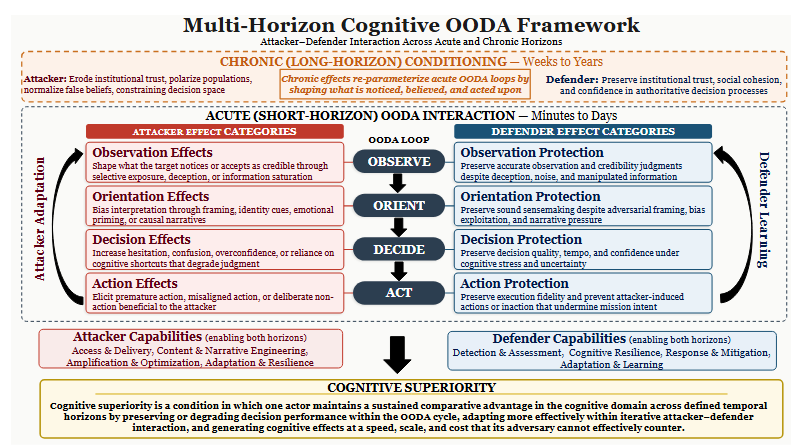
\includegraphics[width=0.95\linewidth]{images/guerra_cognitiva_OODA.png}
\caption{Marco OODA multi-horizonte de la guerra cognitiva \cite{RushingHerschXu2026}. El bucle OODA central articula los efectos del atacante (izquierda) y las protecciones del defensor (derecha) en el horizonte agudo (corto plazo, minutos a días). El horizonte crónico (largo plazo, semanas a años) reconfigura los parámetros del bucle mediante efectos acumulativos sobre creencias y decisiones. La interacción iterativa atacante--defensor determina quién alcanza la superioridad cognitiva.}
\label{fig:ooda}
\end{figure}

Trasladar esta definición a un simulador multiagente requiere fijar la unidad mínima de análisis.
La respuesta que adopta este modelo es inequívoca: \emph{el mensaje es la munición; el blanco, la mente} \cite{Hoffman2025}.
Una operación cognitiva es, en esencia, un flujo de mensajes que altera estados cognitivos; por tanto, el objeto central del modelo no es el agente sino el mensaje que circula entre agentes.

\paragraph{Bucle OODA y horizonte temporal.}
El mecanismo que gobierna la conducta de cada agente sigue el bucle \emph{Observe–Orient–Decide–Act} (OODA) en su variante multi-horizonte \cite{RushingHerschXu2026}, que distingue dos escalas temporales con implicaciones cualitativamente distintas.

El \textbf{horizonte corto plazo} abarca minutos, horas o días: corresponde a la fase aguda de una campaña informativa, en la que la narrativa se difunde rápidamente aprovechando la viralidad de los \emph{hubs} y el contagio emocional antes de que los mecanismos de verificación puedan activarse.
En este horizonte dominan la velocidad de penetración ($t_{50}$), el alcance máximo y la amplitud del pico de nuevas conversiones, junto con las métricas de resultado poblacional: la \textbf{tasa de ataque} $a$ ---fracción de la población que adopta la narrativa--- y la \textbf{resiliencia poblacional} $R = 1 - a$.
Los ataques de corto plazo buscan crear hechos consumados: fijar una versión inicial de los eventos que resulte difícil de desalojar una vez instalada.

El \textbf{horizonte largo plazo} abarca semanas, meses o años: corresponde a la consolidación de la narrativa en las estructuras cognitivas de la población y en la arquitectura de la red.
En este horizonte domina la entropía cognitiva $H$, que mide en qué medida la narrativa ha erosionado la diversidad de creencias de forma estructural y duradera.

El experimento de este trabajo opera exclusivamente en el \textbf{horizonte corto plazo}: la simulación corre durante $45$ pasos equivalentes a tres días de actividad a $15$ pasos/día, donde cada paso representa una hora.
En cada paso cada agente puede procesar y emitir múltiples mensajes, capturando la actividad asíncrona característica del tráfico en redes sociales digitales.
La evaluación del horizonte largo plazo ---consolidación estructural de narrativas, erosión de instituciones--- queda como línea de trabajo futuro.

En cada paso de simulación el agente: (i)~\emph{observa} los mensajes acumulados en su bandeja de entrada (\emph{inbox}); (ii)~\emph{se orienta} actualizando su estado interno; (iii)~\emph{decide} si emite un mensaje nuevo o reenvía alguno de los recibidos; y (iv)~\emph{actúa} depositando el mensaje resultante en su buzón de salida (\emph{outbox}).
Para garantizar determinismo y eliminar condiciones de carrera, el simulador divide cada paso en dos sub-fases secuenciales: \textbf{TX} (todos los agentes ejecutan Decide+Act y pueblan sus \emph{outboxes}) y \textbf{RX} (los mensajes se entregan a los \emph{inboxes} de los destinatarios y se registran en las trazas).
Esta separación asegura que ningún agente procesa en el mismo paso un mensaje que otro acaba de generar, reproduciendo la latencia real de cualquier canal de comunicación.

\paragraph{El mensaje como objeto central.}
El objeto central del modelo es el mensaje, formalizado como una tupla inmutable de doce campos:

\begin{equation}
m = (id,\, trace,\, t,\, src,\, tgt,\, \ell,\, M_{od},\, e,\, \lambda,\, v,\, s,\, parent)
\label{eq:mensaje}
\end{equation}

La Tabla~\ref{tab:mensaje} detalla el dominio y el papel de cada variable.
La \emph{capa} $\ell \in \{\text{analógica},\,\text{digital}\}$ determina la función de confianza aplicable y la modalidad por defecto: la capa analógica corresponde a comunicación presencial (cara a cara), mientras que la digital admite cualquier modalidad.
La \emph{modalidad} $M_{od} \subseteq \{\text{texto},\,\text{audio},\,\text{imagen},\,\text{vídeo}\}$ modula la ganancia de impacto perceptual del mensaje: el vídeo tiene el mayor potencial persuasivo, seguido de audio, imagen y texto, en coherencia con la literatura sobre persuasión multimodal.
La \emph{emoción dominante} $e$ se toma del conjunto de las ocho emociones primarias de Plutchik más la etiqueta neutra \cite{Plutchik1980}; su presencia en el mensaje abre la puerta a modelar contagio emocional sin necesidad de una psicología del agente más elaborada.
La \emph{carga emocional} $\lambda \in [0,1]$ cuantifica la intensidad de esa emoción y constituye el principal driver de persuasión del mensaje: un mensaje puede ser falso y aun así persuadir si su carga emocional es elevada.
La \emph{veracidad percibida} $v \in [0,1]$ no modula directamente la persuasión ---el modelo no asume que los agentes evalúan la verdad--- sino que etiqueta el mensaje como \emph{narrativa} (desinformación) cuando $v \leq v_{thr}$, distinguiéndolo del ruido neutro.
Esta elección está respaldada por la evidencia empírica de que las noticias falsas se difunden significativamente más rápido y más lejos que las verdaderas \cite{Vosoughi2018}.
La \emph{saliencia} $s \in [0,1]$ captura la relevancia subjetiva que el receptor atribuye a la fuente; es el mecanismo por el que las fuentes de autoridad percibida ejercen mayor influencia.
Por último, los campos $trace$ y $parent$ implementan la trazabilidad causal: $trace$ agrupa todos los mensajes de una misma campaña y $parent$ apunta al mensaje del que este es reenvío directo, permitiendo reconstruir el árbol de difusión completo para análisis \emph{post hoc}.

\begin{table}[h!]
\centering
\caption{Variables del mensaje $m$ (ecuación~\ref{eq:mensaje}): símbolo, dominio y papel en el modelo.}
\label{tab:mensaje}
\begin{tabular}{@{}l p{4.2cm} p{8cm}@{}}
\toprule
\textbf{Símbolo} & \textbf{Dominio} & \textbf{Papel en el modelo} \\
\midrule
$id$       & UUID                                           & Identificador único del mensaje \\
$trace$    & UUID                                           & Identificador de campaña; agrupa mensajes relacionados \\
$t$        & $\mathbb{N}$                                   & Paso de simulación en que se emite \\
$src$      & $V$ (nodo del grafo)                           & Agente emisor \\
$tgt$      & $V$ (nodo del grafo)                           & Agente receptor \\
$\ell$     & \{analógica, digital\}                         & Capa; determina función de confianza y modalidad por defecto \\
$M_{od}$   & $\mathcal{P}$(\{texto, audio, imagen, vídeo\}) & Modalidad/canal; modula ganancia de impacto perceptual \\
$e$        & Emociones Plutchik $\cup$ \{neutro\}           & Emoción dominante del mensaje \cite{Plutchik1980} \\
$\lambda$  & $[0,1]$                                        & Carga emocional; intensidad de la emoción del mensaje \\
$v$        & $[0,1]$                                        & Veracidad percibida; etiqueta narrativa si $v \leq v_{thr}$ \\
$s$        & $[0,1]$                                        & Saliencia; relevancia subjetiva atribuida al emisor \\
$parent$   & UUID $\cup$ \{\texttt{None}\}                  & Referencia al mensaje origen (trazabilidad causal) \\
\bottomrule
\end{tabular}
\end{table}

La dinámica emergente del modelo nace de la coexistencia de dos \emph{especies} de mensajes con propiedades opuestas.
La \emph{narrativa} se caracteriza por veracidad percibida baja ($v \leq v_{thr}$) y carga emocional alta ($\lambda \approx 1$): es el vector de desinformación que persuade precisamente porque apela a la emoción y no a la evidencia.
El \emph{ruido neutro}, en cambio, presenta veracidad alta y emoción neutra: no persuade, pero mantiene activo el canal de comunicación y proporciona el ruido de fondo sobre el que la narrativa compite.
Su competencia sobre la misma red genera patrones de difusión no lineales que la simulación permite observar y medir.
La métrica que captura el efecto agregado es la \emph{entropía cognitiva} definida en el marco del \emph{Cognitive Net Assessment} \cite{PolytechniqueCNA2026}: una población con creencias distribuidas de forma más uniforme ---mayor entropía--- es más vulnerable a la narrativa, porque ninguna creencia dominante actúa como ancla colectiva.
Esta métrica operacionalizará el concepto de superioridad cognitiva en la fase de análisis de resultados, cerrando el ciclo entre el marco teórico y el diseño computacional del simulador.
